
\chapter{The distributive property}

The distributive law will be the star of the tensor show.   Distributive laws
appear throughout our world of measurement and this offers some gentle points 
of entry to the study.  
Start with area.
\begin{center}
    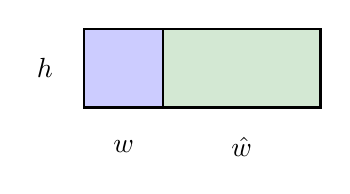
\begin{tikzpicture}
        \draw[thick, fill=blue!20] (0,0) rectangle (1,1);
        \draw[thick, fill=ForestGreen!20] (1,0) rectangle (3,1);

        \node at ( 0.5,-0.5) {$w$};
        \node at ( 2,-0.5) {$\hat{w}$};
        \node at (-0.5,0.5) {$h$};

    \end{tikzpicture}
\hspace{1in}
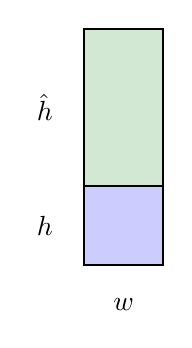
\begin{tikzpicture}
    \draw[thick, fill=blue!20] (0,0) rectangle (1,1);
    \draw[thick, fill=ForestGreen!20] (0,1) rectangle (1,3);

    \node at ( 0.5,-0.5) {$w$};
    \node at (-0.5,0.5) {$h$};
    \node at (-0.5,2) {$\hat{h}$};

\end{tikzpicture}
\end{center}
So area as  function $A(w,h)$ of width and height distributes over those parameters.
\begin{align*}
    A(w+\hat{w},h) &= A(w,h)+A(\hat{w},h)
    &    A(w,h+\hat{h}) &= A(w,h)+A(w,\hat{h})
\end{align*}
Calculus says that all areas are defined by distributed sums 
of subrectangles, or by the steady approximation by such rectangles.
Thus area's distributive property water-marks calculus 
in numerous ways including the following fundamental identity.
\begin{align*}
    \int_M (f+g)\text{d}x = \int_M f \text{d}x + \int_M g \text{d}x
\end{align*}

\subsection{``Real'' life}
Look elsewhere in your life.  When you buy $x$ items at cost $\text{Cost}(x)$
and then buy $\acute{x}$ more the total cost is:
\[
    \text{Cost}(x+\acute{x})=\text{Cost}(x)+\text{Cost}(\acute{x}).
\]  
Add the cost of tax $\text{Tax}(x)$ and the total changes to 
\[
    (\text{Cost}+\text{Tax})(x)=\text{Cost}(x)+\text{Tax}(x).
\]
It is not just cost of one item.  Buy items $x_1,\ldots, x_n$ at 
costs $C_i(x_i)$ each and set 
\(
    \text{Cost}(x_*)=\text{Cost}(x_1,\ldots,x_n) = C_1(x_1)+\cdots +C_n(x_n)
\)
Still we find
$\text{Cost}(x_*+\acute{x}_*)=\text{C}(x_*)+\text{Cost}(\acute{x}_*)$.
Cost distributes.  

Here is another life situation.  The work of $e$ employee for $h$ hours produces 
$\text{W}(e,h)$ widgets
so at peak productivity adding $\hat{e}$ workers or $\hat{h}$ extra hours we get
\begin{align*}
    \text{W}(e+\hat{e},h)& =\text{W}(e,h)+\text{W}(\hat{e},h)
    &
    \text{W}(e,h+\hat{h})& =\text{W}(e,h)+\text{W}(e,\hat{h}).
\end{align*}
Work distributes, both over workers and over time.

% Imagine next the ingredient list 
% $\text{Supplies}(r)$ of recipe $r$.  If we need to shop for ingredients of two recipes 
% $r$ and $\acute{r}$ then 
% \[
%     \text{Supplies}(r+\acute{r})=\text{Supplies}(r)+\text{Supplies}(\acute{r}).
% \]
Need to print the names of both faculty and graduate students. 
You could distribute that work as well, as seen in Listing~\ref{lst:distributive},
the command \code{Print} distributes over the operator of concatenation \code{cat}
with the result of simply appending the two individual printing commands.
We could say 
\begin{center}
    \code{Print(as cat bs) == Print(as) append Print(bs)}
\end{center}

\begin{lstfloat}
\begin{notebookin}
fac = [ "Hamilton", "Levi-Chivita" ]
students = [ TBD use math geoneolgoy to find some students of these]
Print(faculty cat students)
\end{notebookin}
\begin{notebookout}
Hamilton
Levi-Chivita
....TBD
\end{notebookout}
\begin{notebookin}
Print(faculty)
Print(students)
\end{notebookin}
\begin{notebookout}
Hamilton
Levi-Chivita
....TBD
\end{notebookout}
\caption{Many operations in computation are distributive.}\label{lst:distributive}
\end{lstfloat}

Well all this is at least true for some range of values.  All scientific
claims of connection to reality are true only for sensible regions of values.

The distributive appears so often because we are willing to be flexible about 
what we want from addition and multiplication.  We just use those two names 
to remember ``multiplication distributes over addition''---whatever those two 
terms mean.

\subsection{Notations}

By custom, area $A(w,h)$ of rectangles is denoted $w \cdot h$ and called
multiplication.  In that notation we have the familiar form.
\begin{align*}
    (w+\hat{w})\cdot h & = w \cdot h +\hat{w}\cdot h 
    &
    w\cdot (h+\hat{h}) & = w\cdot h + w\cdot \hat{h}.
\end{align*}
This is the first of dozens of notations invented over the centuries to communicate 
functions that distribute their work amongst sums of sub-applications of the function.  
Most honor one of these three modes:
\begin{itemize}
    \item functions on the outside applied to sums of inputs 
    \[ 
        f(u+\acute{u})=f(u)+f(\acute{u}),\qquad 
        \code{Print(as cat bs)},\qquad
        \text{Cost}
        (x,y,z)\ldots;
    \]

    \item functions in the middle like these operators 
    \[
        (u+\acute{u})*v=u*v+\acute{u}*v, \qquad 
        (u+\acute{u})\cdot v=u\cdot v+\acute{u}\cdot v,\qquad 
        u\otimes v, \qquad 
        uv,\ldots; 
    \]

    \item functions on the outside like these
    \[
        \langle u+\acute{u}|v\rangle=\langle u|v\rangle +\langle \acute{u}|v\rangle,\qquad 
        [u+\acute{u},v]=[u,v]+[\acute{u},v],\qquad  
        /u,v/,\ldots~.
    \]
    
\end{itemize}
   
\subsection{Axes and dependent-functions}
Just, as area distributes, so does volume $V(\ell,w,h)$ only with one more axis.
\begin{center}
    \textbf{[TBD: a tikz picture of three volumes showing three axes of distributive volume]}
\end{center}
As formulas this could be written:
\begin{align*}
    V(\ell+\hat{\ell},w,h) & = V(\ell,w,h)+V(\hat{\ell},w,h)\\
        V(\ell,w+\hat{w},h) & = V(\ell,w,h)+V(\ell,\hat{w},h)\\
        V(\ell,w,h+\hat{h}) & = V(\ell,w,h)+V(\ell,w,\hat{h})
\end{align*}
With volumes we obviously must give up on the chiral language of ``distributes on the left''
``distributes on the right''.   Venturing into hypervolumes will be worse and benefits from some notation.  

First we need to name every coordinate and while we could number coordinates 
a for more flexible idea is the name them after what they mean.  For example 
the rows and columns of matrix are typically used in that order and rows 
are interpreted as moving top-to-bottom..  Meanwhile $x$ and $y$ flip this 
convention with the left-to-right going first and bottom-to-top orientation for 
vertical.  So a function $M_{rc}$ in row-column form is differently interpreted 
from a function $f_{xy}$ in $x$-axis, $y$-axis form.  So naming the axes 
rather than prescribing fixed meaning is the most common.

Now that the axes $A$ are named, when we want to changing value $x_a$ on an axis $a\in A$ 
we do so merely by providing an annotation, usually a subscript.
For example $A=\{\text{row},\text{col}\}$ means we could consider 
$u_A=(u_{\text{row}}, u_{\text{col}})$.  What is going on here is that we are not actually
describing an ordered pair but instead a function whose output type depends on the input
or what is more commonly known as a \emph{dependent-function}.  Order-pairs 
can be seen as special cases of dependent -functions, they depend on $A=\{\text{left},\text{right}\}$
or sometimes $\{1,2\}$, but the the convention for writing ordered pairs $(x,y)$ is that the 
position of the value is fixed and from that one recovers the implicit input, e.g. $x$ is in the left 
so implicitly $\text{left}\mapsto x$.

There are two notations used somewhat interhcangeably for dependent-functions
\begin{align}
    u_A & :a\mapsto u_a & 
    u_A & = (u_a\mid a\in A)
\end{align}
When it become tedious we write $u=u_A$.
If we partition $A=B\sqcup C$ we can accordingly restrict the dependent-function $u$ 
to the smaller domains creating two dependent-functions $u_B$ and $u_c$ with the same overall information,
which we write
\begin{align*}
    u_A & = (u_B, u_C)
\end{align*}
An especially important case is for $a\in A$ where we let $\bar{a}=A-\{a\}$ and write 
\begin{align*}
    u_A & = (u_a,u_{\bar{a}})
\end{align*}

Back to volume we could now have stated $A=\{\text{l},\text{w},\text{h}\}$ as the axes.
Then volume is a function $\text{Vol}(u_A)$ where for each $a\in A$, $u_a\geq 0$.  Thus 
the distributive property in all three variables can be condensed to a single formula 
quantified over every axis.
\begin{align*}
    & (\forall a\in A)
    &
    \text{Vol}(u_{a}+\acute{u}_a,u_{\bar{a}}) & = \text{Vol}(u_a,u_{\bar{a}}) + \text{Vol}(\acute{u}_a,u_{\bar{a}}) 
\end{align*}
Notice if we change $A=\{\text{w},\text{h}\}$ we get the distributive law for area, 
and if we change to $A=\{x,y,z\}$ we get volume but no in reference to xyz-coordinates
instead of the more ambiguous length-width-height coordinates.  Hypervolumes are 
then the same rule but with more axes such as $A=\{x,y,z,t\}$ or axes $A=\{x_1,\ldots, x_{\ell}\}$.

\emph{In these notes $u_A=(u_a\mid a\in A)$ denotes a dependent-function not an ordered tuple.}

\section{Distributive algebra}


What does distribution require?
\begin{align}
    u*(v+\acute{v}) & = u*v+u*\acute{v}
    & 
    (u+\acute{u})*v & = u*v + \acute{u}*v.
\end{align}
We definitely need additions, but we should not jump to assume that $u$, $v$, and $w$ are 
of the same type of data.  Just look at  matrix 
multiplication (we use $\mathbb{R}^{a\times b}$ to denote $(a\times b)$-matrices 
of real numbers)
\begin{align*}
    *&:\mathbb{R}^{a\times b}\times \mathbb{R}^{b\times c}\to \mathbb{R}^{a\times c}
    &
    (u*v)_{ij} & = \sum_k u_{ik}v_{kj}.
\end{align*}
So we except this is a study of \emph{heterogeneous} algebra, so we wont be
captivated by homomorphism but rather what we will call \emph{hetero}morphisms.
So we could think of three types of data $U$, $V$ and $W$ each with a $+$ each
combined by a function 
$*:U\times V\to W$
that satisfies the distributive law.  Because this is the start it will get its own 
notation, we write $\bmto$, that is 
\begin{align*}
    *:U\times V\bmto W
\end{align*}
denotes a distributive function on additive structures $U$, $V$, and $W$.
As we go along we will prefer to use $U$, $V$ and $W$ in just this way so that 
we can get up to speed on examples as quickly as possible.


\subsection{Properties of addition}
It is tempting now to start  assuming that $U$, $V$, and $W$ are 
something family---vector spaces, modules, or at least abelian groups.
However this would rob the distributive law of its power and leave us to think 
addition and its common attributes are the reason tensors work.  But the 
distributive law is already claiming a strong interaction of two operations 
so maybe it should be explored on its own a little while longer to appreciate 
what it already says about the individual operations.  More examples will demonstrate 
the value of a general point of view.

We will use a number of spaces
\begin{align*}
    \mathbb{R}^d & \defeq \{u:[d]\to \mathbb{R}\},\\
    R^{m\times n} &\defeq \{M:[m]\times [n]\to \mathbb{R}\}\\
    R^{\ell\times m\times n} &\defeq \{\Gamma:[\ell]\times [m]\times [n]\to \mathbb{R}\}\\
    & \vdots
\end{align*}
Define the following operations.
\begin{gather*}
    \mathbb{R}^m\oplus \mathbb{R}^n  \defeq \mathbb{R}^{m+n}\\
    \begin{bmatrix} \mathbb{R}^{a\times n} \\ \mathbb{R}^{b\times n} \end{bmatrix} \defeq \mathbb{R}^{(a+b)\times n}
    \qquad
    \begin{bmatrix}
    \mathbb{R}^{m\times c} &
    \mathbb{R}^{m\times d}
    \end{bmatrix}  \defeq \mathbb{R}^{m\times (c+d)}\\
%     \mathbb{R}^{a\times m\times n} \oplus \mathbb{R}^{b\times m\times n}  \defeq \mathbb{R}^{(a+b)\times m\times n}
%     \qquad
%     \mathbb{R}^{\ell \times c\times n} \oplus \mathbb{R}^{\ell \times d\times n}  \defeq \mathbb{R}^{\ell\times (c+d)\times n}
%     \qquad
% \\  
%      \mathbb{R}^{\ell \times m\times e} \oplus \mathbb{R}^{\ell \times m\times f}  \defeq \mathbb{R}^{\ell\times m\times (e+f)}\\
     \vdots
\end{gather*}



Now we add a multiplication.
\begin{align*}
    \mathbb{R}^m \otimes \mathbb{R}^n & \defeq \mathbb{R}^{m\times n}
\end{align*}

\begin{example}
    The distributive law with vector space operators.
    \begin{align*}
    (\mathbb{R}^a \oplus \mathbb{R}^b)\otimes \mathbb{R}^n 
        % & = \mathbb{R}^{(a+b)\times c}
        &  = \begin{bmatrix}\mathbb{R}^{a}\otimes \mathbb{R}^n  \\ \mathbb{R}^b\otimes \mathbb{R}^n\end{bmatrix}\\
    \mathbb{R}^m\oplus ( \mathbb{R}^c \oplus \mathbb{R}^d )
        % & = \mathbb{R}^{(a+b)\times c}
        &  = \begin{bmatrix} 
            \mathbb{R}^{m}\otimes \mathbb{R}^c &
            \mathbb{R}^m\otimes \mathbb{R}^d
        \end{bmatrix}
    \end{align*}
\end{example}

Lets combine the left and right 
distributive laws.

\begin{center}
    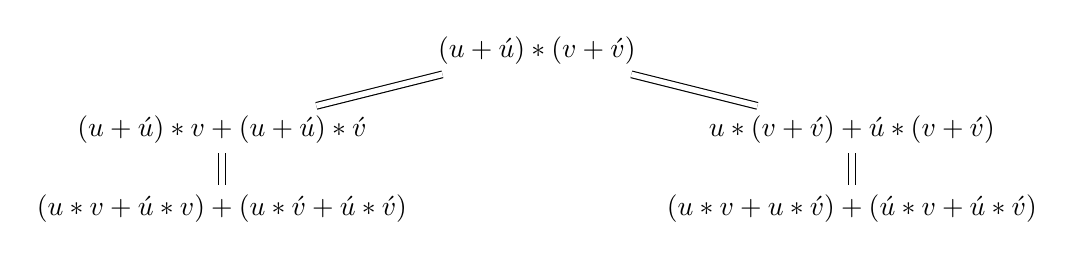
\begin{tikzpicture}[xscale=2]
        \node (A) at (0,0) {$(u+\acute{u})*(v+\acute{v})$};
        \node (B) at (-2,-1) {$(u+\acute{u})*v+(u+\acute{u})*\acute{v}$};
        \node (C) at (2,-1) {$u*(v+\acute{v})+\acute{u}*(v+\acute{v})$};
        \node (D) at (-2,-2) {$(u*v+\acute{u}*v)+(u*\acute{v}+\acute{u}*\acute{v})$};
        \node (E) at (2,-2) {$(u*v+u*\acute{v})+(\acute{u}*v+\acute{u}*\acute{v})$};
        \draw[double distance=2pt] (A) -- (B);
        \draw[double distance=2pt] (A) -- (C);
        \draw[double distance=2pt] (B) -- (D);
        \draw[double distance=2pt] (C) -- (E);
    \end{tikzpicture}
\end{center}
Thus the values $a,b,c,d,\ldots $ in the image of a distributive product $*:U\times V\bmto W$ must 
satisfy the following identity.
\begin{equation}
    \tag{Distributable}
    (a+b)+(c+d) = (a+c)+(b+d)
\end{equation}

\begin{proposition}
    If $+$ is both associative and commutative then it is distributable.
    Furthermore, such an addition can be extended to have at $0$.

    Conversely, if $+$ is distributable and has a $0$ then $+$ is associative 
    and commutative.
\end{proposition}
\begin{proof}
    TBD
\end{proof}

\subsection{Formulas and subalgebras}
We are in a territory where we are assuming very little about our addition 
so that we leave open the possiblity of applying the ideas of tensors broadly.
This already included examples where the data we add include things like vector spaces,
and there is no ``set of all vector spaces''.  In fact sets themselves are a bit 
of mismatch with algebra.  This causes no trouble.  Algebra predates sets 
(think of Boolean, Heyting and de Morgan algebra) and outlasts sets (think 
of categories).  If this makes you uncomfortable you should note that programming 
is in the same boat.  It describes logic outside of sets all the time.
So what is algebra without sets?  Well what is math without sets! 
It takes a step back and becomes all about language.  In otherwords 
it is time to go back to grammar school.

We want additive structures so we use $+$ and we want that be $x+y$, because 
at least for math 
styles like $+x~y$ or \code{add(x,y)} are not our preference.
To feel sophisticated about this we could report that we have the following 
grammar:
\begin{center}
\begin{lstlisting}
<A>::= (<A>+<A>) | 0
\end{lstlisting}   
\end{center}
where $|$ indicates ``or'' and so we can add or use $0$.  If we do not want 
$0$ in our addition we just remove it; likewise, if wish to add something like 
negatives we can add this as well as in the following.
\begin{center}
\begin{lstlisting}
<An>::= (<AN>+<AN>) | 0 | -<AN>
\end{lstlisting}   
\end{center}


We will want some formulas.  So we add variables, 
for examples to add $X=\{x,y,z\}$ as variables we use
\begin{center}
\begin{lstlisting}
   <X> ::= x | y 
<A<X>> ::= <X> | 0 |(<A<X>>+<A<X>>)      
\end{lstlisting}
\end{center}


Strings $\Phi:=\Phi(X)$ that prase in this grammar are called \emph{additive formulas} 
and annotated $\Phi:\text{Fr}_{A}\langle X\rangle$.  For example 
$((x+0)+y):\text{Fr}_A\langle x,y\rangle$, 
but not $+xy$ because that does not match the pattern in the grammar.

Given an additive structure $W$ and assignment of variables $w_X:W^X$
we can substitute into a formula $\Phi(X)$ the values $w_X$ formula 
a list of operations to carry out in $W$ called \emph{evaluation} and denoted 
$\Phi(w_X)$.  For example $\Phi(x,y)=((x+0)+y)$ and $W=\mathbb{N}$ then 
$\Phi(2,3)=((2+0)+3)=5$.  

Now given an additive algebra $W$ and a function $S:I\to W$, then 
the evaluations $\Phi(s_*)$ are said to have type 
\begin{align*}
    \text{Fr}_{+,0}\langle S\rangle 
\end{align*}
We say that $\text{Fr}_{+,0}\langle S\rangle$ is the subalgebra generated 
by $S$.

\subsection{Congruence, quotients, \& homomorphisms}
Algebra is the study of equations with variables, e.g.\ $x^2+1=0$.  
The most general form of algebra should allow every symbol to vary.  
So we can replace $+$ one day with addition of decimal numbers, 
the next day $+$ is addition of complex.  Later we are adding matrices
or polynomails etc.  The $+$ is changing.  But so too is the $=$. 
Equality of decimals is not equality of matrices.  The theory of 
changing equality is Noether's Isomorphism theorem.  To get there let 
us recall an even more basic resonance.

\begin{theorem}[Resonance Theorem]
    In a calculus of constructions
    \begin{center}
        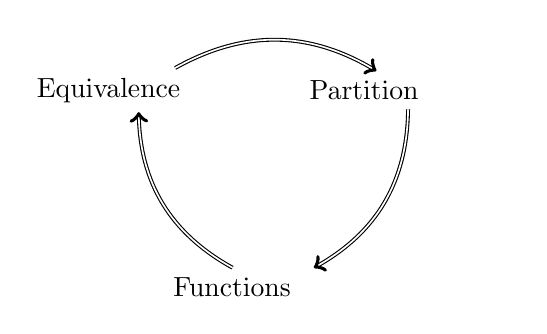
\begin{tikzpicture}
            \node[text width=1in] (EQ) at (150:2) {Equivalence};
            \node[text width=1in] (Part) at (30:2) {Partition};
            \node[text width=1in] (Fib) at (270:1.5) {Functions};

            \draw (EQ) edge[->, double, bend left] (Part);
            \draw (Part) edge[->, double, bend left] (Fib);
            \draw (Fib) edge[->, double, bend left] (EQ);
        \end{tikzpicture}
    \end{center}
\end{theorem}

Now we add algebra to the data and select those equivalence relations that respect the algebra.
Equivalence relations that respect algebra are called \emph{congruences}.
By convention a congruence relation $R$ is denoted as 
\[  
    a\equiv\acute{a}\pod{R}
\]
where $R$ is the name of the congruence.
\begin{example}
    In a $\{+,0,-\}$-algebra,
    \[
        \begin{array}{crcl}
            & a & \equiv & \acute{a} \pod{R}\\
        + &  b & \equiv & \acute{b} \pod{R}\\
        \hline 
            & a+b & \equiv & \acute{a}+\acute{b}\pod{R}
        \end{array}
        \qquad 
        \begin{array}{rcl}
            \\
            \\
        \hline 
            0 & \equiv& 0 \pod{R}
        \end{array}
        \qquad 
        \begin{array}{crcl}
            \\
        -   & a & \equiv & \acute{a} \pod{R}\\
        \hline 
            &  -a & \equiv & -\acute{a} \pod{R}
        \end{array}
    \]
    Of course operators that depend on no parameters---0-valent operators---are 
    trivially respected by all equivalence relations, but we include these 
    in the list to make it clear that every operator is being considered.
\end{example}

A partition $\{[a]\mid a\in A\}$ of an algebra that respects the operations is called a \emph{quotient}.
For instance for a $\{+,0,-\}$-algebra the partition would mean the following are well-defined.
\begin{align*}
    [a]+[b] & = [a+b] 
    & 
    [0] & = [0] 
    &
    -[a] & = [-a].
\end{align*}
By convention, quotients $\mathcal{P}$ are denoted $A/\mathcal{P}$ and the classes $[a]$, which we denote 
by $a/\mathcal{P}$, are called \emph{cosets} (even when they are not sets).

Finally a function $\varphi:A\to B$ between algebras that respects operations of (homogeneous) algebra $A$ will called a 
\emph{homomorphism} and to complete the example here is what respect means for $\{+,0,-\}$-algebras.
\begin{align*}
    \varphi(a+\acute{a}) & = \varphi(a)+\varphi(\acute{a})
    & 
    \varphi(0) & = 0
    &
    \varphi(-a) & = -\varphi(a).
\end{align*}
Now we update the resonance to match.

\begin{theorem}[Noetherian Resonance]
    In a Martin-L\"of typed algebra
    \begin{center}
        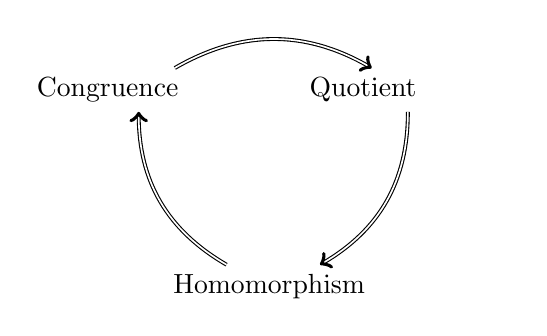
\begin{tikzpicture}
            \node[text width=1in] (EQ) at (150:2) {Congruence};
            \node[text width=1in] (Part) at (30:2) {Quotient};
            \node[text width=1in] (Fib) at (270:1.5) {Homomorphism};

            \draw (EQ) edge[->, double, bend left] (Part);
            \draw (Part) edge[->, double, bend left] (Fib);
            \draw (Fib) edge[->, double, bend left] (EQ);
        \end{tikzpicture}
    \end{center}
\end{theorem}
\begin{proof}
    From congruences to quotients use:  
    \begin{center}
        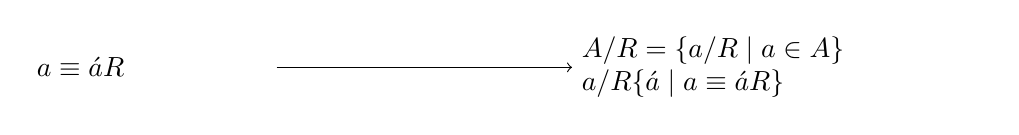
\begin{tikzpicture}
            \node[text width=1.15in] (EQ) at (0,0) {$a\equiv \acute{a}\pod{R}$};
            \node[text width=2in] (Part) at (8,0) {$A/R=\{a/R\mid a\in A\}$\\ $a/R\defeq \{\acute{a}\mid a\equiv \acute{a}\pod{R}\}$};
            \draw (EQ) edge[->, ] (Part);
        \end{tikzpicture}
    \end{center}
    
    From quotients to homomorphisms use:  
    \begin{center}
        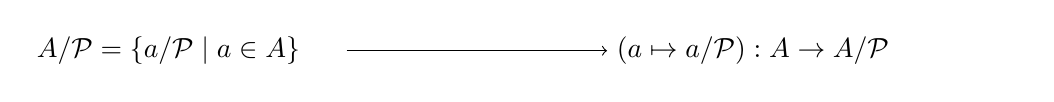
\begin{tikzpicture}
            \node[text width=1.5in] (EQ) at (0,0) {$A/\mathcal{P}=\{a/\mathcal{P}\mid a\in A\}$};
            \node[text width=2in] (Part) at (8,0) {$(a\mapsto a/\mathcal{P}):A\to A/\mathcal{P}$};
            \draw (EQ) edge[->, ] (Part);
        \end{tikzpicture}
    \end{center}

    From homomorphism to congruence use kernels.
    \begin{center}
        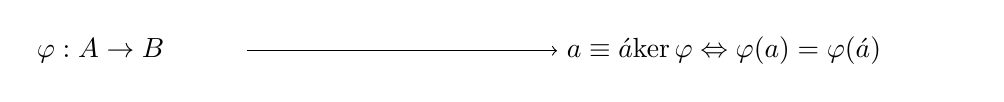
\begin{tikzpicture}
            \node[text width=1in] (EQ) at (0,0) {$\varphi:A\to B$};
            \node[text width=2in] (Part) at (8,0) {$a\equiv \acute{a} \pod{\ker \varphi} \Leftrightarrow \varphi(a)=\varphi(\acute{a})$};
            \draw (EQ) edge[->, ] (Part);
        \end{tikzpicture}
    \end{center}

\end{proof}


\subsection{Distributable \& Commonoids}

Now we get to tame the algebra.  
\begin{definition}
    Given a distributive product $*:U\times V\bmto W$
    let 
    \begin{align*}
        (u\equiv \acute{u} \pmod{V^{\top}}) & \Leftrightarrow (\forall v\in V)(u*v=\acute{u}*v)\\
        (v\equiv \acute{v} \pmod{U^{\bot}}) & \Leftrightarrow (\forall u\in U)(u*v=u*\acute{v})\\
        U*V & := \text{Fr}_{+,0}\langle u*v \mid u\in U, v\in V\rangle
    \end{align*}
    When necessary we denoted equivalence classes $u/{V^{\bot}}$ and etc.
\end{definition}

\begin{proposition}
    Each of the following induced products are well-defined and distributive.
    \begin{itemize}
        \item $*:U/V^{\top} \times V\bmto W$
        \item $*:U \times V/U^{\bot}\bmto W$
        \item $*:U \times V\bmto W^+$
        \item $*:U/V^{\top} \times V/U^{\bot}\bmto U*V$
    \end{itemize}
\end{proposition}
\begin{proof}
    TBD by a Wilsonite
\end{proof}

\begin{definition}
    An additive algebra that is both associative and commutative is called a \emph{commonoid}.
\end{definition}

\begin{proposition}
    Given a distributive product $*:U\times V\to W$ then 
    $U/V^{\bot}$, $V/U^{\top}$ and $W^+=U*V$ are commonoids.
\end{proposition}
\begin{proof}
    TBD by a Wilsonite
\end{proof}

\subsection{Grothendieck group}

\begin{theorem}
    If $M$ is a commonoid then 
    \begin{align*}
        (m,n) \equiv (\acute{m},\acute{n}) \pod{Grth} & \Leftrightarrow (\exists k\in M)(m+\acute{n}+k=\acute{m}+n+k)
    \end{align*}
    is a congruence on $M\oplus M$.  Furthermore,
    \begin{align*}
        (m,n)+(n,m) \equiv (0,0) \pod{Grth}
    \end{align*}
    So $\Gr(M)\defeq M\oplus M/Grth$ is an abelian group where 
    \[
        -(m,n)\defeq (n,m)
    \]
    This is called the Grothendieck group of $M$.
    The interpretation is that $(m,n)/R$ is ``m-n''.  When $m=0$ it is customary to write $-n$.

    The homomorphism $M\to \Gr(M)$ given by $m\mapsto (m,0)$ is injective 
    if, and only if, $m+n=m+\acute{n}$ implies $m=m$, i.e.\ $M$ has cancellation.
\end{theorem}

\begin{proposition}
    If $u\in U$ with $-u$ such that $u+(-u)=0$ then 
    \[
        u*v + (-u)*v =0
    \]
    Thus if $U$ has negatives then we can promote these negatives to $U*V$.
    In particular $-(u*v)\defeq (-u)*v$ defines a negative in $W$ of $u*v$.
    We can do likewise in the variable $V$.  
\end{proposition}
Now imagine the distributive law was present along side an existing subtraction.
Then the following would be a consequence.
\begin{align*}
    (a-b)*(c-d) & = (a*(c-d))-(b*(c-d))
        = (a*c-a*d)-(b*c-b*d)\\
        & =(a*c+b*d)-(a*d+b*c)
\end{align*}
This should explain the following extension.

\begin{corollary}
    If $*:U\times V\bmto W$ is a distributive product of commonoids then there is an 
    induced distributive product 
    \begin{gather*}
        * :\Gr(U)\times \Gr(V)\bmto \Gr(W)\\
        (u-\acute{u})*(v-\acute{v})
        \defeq (u*v+\acute{u}*\acute{v})-(u*\acute{v}+\acute{u}*v).
    \end{gather*}
    In particular $(-u)*v=-(u*v)=u*(-v)$.
\end{corollary}

Let us stand back to see what we have built.

\begin{center}
    \begin{tikzcd}
        U\arrow[d,two heads] &[\elastic] 
        \times &[\elastic]
        V\arrow[d,two heads] \arrow[r,"*",tail] &
        W & (\text{Additive algebras})
      \\
        U/V^{\top}\arrow[d] &
        \times &
        V/U^{\bot}\arrow[d] \arrow[r,"\bullet",tail] &
        U*V\arrow[u,hook,"h"]\arrow[d]
        & (\text{Commonoids})\\
        \Gr(U/V^{\top}) &
        \times &
        \Gr(V/U^{\bot}) \arrow[r,"\bullet",tail] &
        \Gr(U*V)
        & (\text{Abelian Groups})
      \end{tikzcd}
    % \begin{tikzcd}
    %     $U$ &[\elastic] $\times$ &[\elastic] $V$ \arrow[tail,r] & $W$\\
    % \end{tikzcd}
\end{center}
It is not a mistake that in the last component the arrows are not aligned.
This is actually a symptom of an unresolved problem in the study of tensors.
They do not lie in a single category.  